% Sets page margins to 1", which is the academic standard
% allows the included extensions of graphic files
% sets graphic path, does not currently work because of space in folder name
% I do not remember what this does
% allows the xhead parameters (text on the top right/left areas of pages)
% \setcounter{tocdepth}{the number of depth}
% INCLUDEGRAPHICS EXPLANATION
% \includegraphics[scale=1]{name of file}
% sometimes you want to twice encase the filename in squiggly brackets. I do not know why but sometimes it is required.
%\setcounter{secnumdepth}{-1}
% \graphicspath{{D:/Dropbox/Private/FP/Gruppe34/FellesDoc/Database/}}


\documentclass{article}
%%%%%%%%%%%%%%%%%%%%%%%%%%%%%%%%%%%%%%%%%%%%%%%%%%%%%%%%%%%%%%%%%%%%%%%%%%%%%%%%%%%%%%%%%%%%%%%%%%%%%%%%%%%%%%%%%%%%%%%%%%%%%%%%%%%%%%%%%%%%%%%%%%%%%%%%%%%%%%%%%%%%%%%%%%%%%%%%%%%%%%%%%%%%%%%%%%%%%%%%%%%%%%%%%%%%%%%%%%%%%%%%%%%%%%%%%%%%%%%%%%%%%%%%%%%%
\usepackage{geometry}
\usepackage{fancyhdr}
\usepackage[pdftex]{graphicx}

%TCIDATA{OutputFilter=LATEX.DLL}
%TCIDATA{Version=5.50.0.2953}
%TCIDATA{<META NAME="SaveForMode" CONTENT="1">}
%TCIDATA{BibliographyScheme=Manual}
%TCIDATA{Created=Monday, January 30, 2012 17:20:46}
%TCIDATA{LastRevised=Monday, March 26, 2012 10:40:20}
%TCIDATA{<META NAME="GraphicsSave" CONTENT="32">}
%TCIDATA{<META NAME="DocumentShell" CONTENT="Standard LaTeX\Blank - Standard LaTeX Article">}
%TCIDATA{CSTFile=40 LaTeX article.cst}

\newtheorem{theorem}{Theorem}
\newtheorem{acknowledgement}[theorem]{Acknowledgement}
\newtheorem{algorithm}[theorem]{Algorithm}
\newtheorem{axiom}[theorem]{Axiom}
\newtheorem{case}[theorem]{Case}
\newtheorem{claim}[theorem]{Claim}
\newtheorem{conclusion}[theorem]{Conclusion}
\newtheorem{condition}[theorem]{Condition}
\newtheorem{conjecture}[theorem]{Conjecture}
\newtheorem{corollary}[theorem]{Corollary}
\newtheorem{criterion}[theorem]{Criterion}
\newtheorem{definition}[theorem]{Definition}
\newtheorem{example}[theorem]{Example}
\newtheorem{exercise}[theorem]{Exercise}
\newtheorem{lemma}[theorem]{Lemma}
\newtheorem{notation}[theorem]{Notation}
\newtheorem{problem}[theorem]{Problem}
\newtheorem{proposition}[theorem]{Proposition}
\newtheorem{remark}[theorem]{Remark}
\newtheorem{solution}[theorem]{Solution}
\newtheorem{summary}[theorem]{Summary}
\newenvironment{proof}[1][Proof]{\noindent\textbf{#1.} }{\ \rule{0.5em}{0.5em}}
\geometry{left=1in,right=1in,top=1in,bottom=1in} 
\DeclareGraphicsExtensions{.pdf,.png,.jpg}
\graphicspath{{E:/Dropbox/Private/FP/Gruppe34/FellesDoc/Database/}}
\setlength{\headheight}{15.2pt}
\pagestyle{fancy}
\lhead{Group 34}
\rhead{FP: DB1}
\input{tcilatex}
\begin{document}


% begin title page, use \\ for newline
\begin{titlepage}
\title{Collaboration Project\\
\textbf{Conceptual Datamodel}\\
Gruppe 34}
% now one can list the authors, \textbf{} makes bold text
\author{Bj\o rn \AA ge Tungesvik\and Tina Syversen\and Andr\'e Philipp\and Odd Magnus Trondrud\and Eivind Kvissel\and H\aa vard H\o iby}
\maketitle
\end{titlepage}

\bigskip

\section{EER-Diagram}

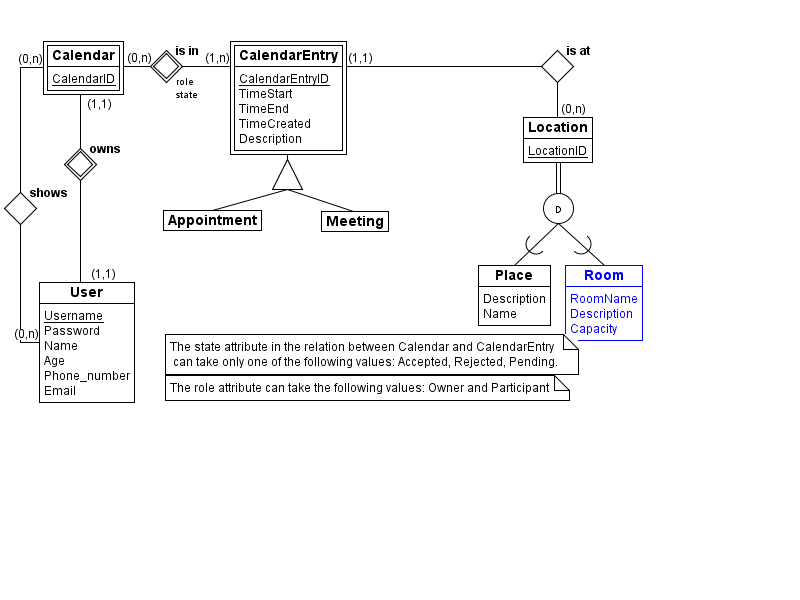
\includegraphics[scale=0.75]{EER_diagram.png} \newpage

\section{Compliance to the Requirement Specifications}

The requirements' description is not presented in this document. The numbers
correspond to the ones found in section 2.2 of the compendium. The rest of
this document is in Norwegian. Sorry about that.

\subsection{Logg p\aa }

Databasen inneholder informasjon som kan verifisere brukere (Username
Password) under User tabellen, s\aa\ personer som logger p\aa\ f\aa r sin
egen User-rad assosiert med den sesjonen.

\subsection{Legge inn avtale}

En avtale legges inn p\aa\ avtaledato med et start- og sluttidspunkt, samt
en kort beskrivelse av avtalen ("Bil p\aa\ verksted") og eventuelt sted for
avtalen ("Strandveien Auto").

CalendarEntry tabellen inneholder felt for start- og slutttidspunkt, felt
for beskrivelse (Henholdsvis TimeStart, TimeEnd og Descripton feltene), og
en relasjon til en tabell kalt Location for \aa\ holde orden p\aa\ sted.
(Sted ligger i Place tabellen som er subklasse til Location)Hver
CalendarEntry rad er knyttet til den spesifikke brukeren som oppretter raden.

\subsection{Slette avtale}

Hver avtale er representert som en CalendarEntry i databasen. En bruker skal
ha full kontroll over avtaler som han har laget, inkludert \aa\ slette dem.

\subsection{Endre avtale}

En bruker skal kunne g\aa\ inn i og endre (gjennom GUI'et)\ hvert felt
bortsett ifra \textquotedblleft timeCreated\textquotedblright\ i
CalendarEntry og Location.

\subsection{Kalle inn til m\o te}

En User skal kunne oprette en rad i Meeting tabellen p\aa\ samme m\aa te som
en avtale, og bli satt som \textquotedblleft leader\textquotedblright\ for
\textquotedblleft Role\textquotedblright\ feltet i \textquotedblleft Is
in\textquotedblright\ - relasjonen mellom Calendar og CalendarEntry, og
bruke \textquotedblleft Owns\textquotedblright\ relasjonen mellom User og
Calendar. Han skal ogs\aa\ kunne invitere andre til m\o tet, de skal bli
satt som \textquotedblleft Participant\textquotedblright\ i
\textquotedblleft Role\textquotedblright\ feltet i \textquotedblleft Is
in\textquotedblright\ relasjonen. Kun den som har \textquotedblleft
Leader\textquotedblright\ i Role i \textquotedblleft is
in\textquotedblright\ relasjonen skal kunne endre feltene innenfor m\o tet.
CalendarEntry - objektet skal ogs\aa\ ha en liste over alle som er assosiert
med m\o tet.

\subsection{Motta m\o teinnkalling}

\textquotedblleft State\textquotedblright\ feltet innenfor \textquotedblleft
Is in\textquotedblright\ relasjonen mellom Calendar og CalendarEntry
tabellen holder orden p\aa\ statusen for de som er assosiert med m\o te.
Dette felte skal bare kunne endres av deltakere i et m\o te, men skal kunne
sees av alle som er innkalt

\subsection{Endre m\o teinnkalling}

N\aa r lederen for en CalendarEntry endrer datoen for m\o te, skal det
sendes ut en beskjed, og en melding om \aa\ oppdatere \textquotedblleft
state\textquotedblright\ til alle assosiert med m\o tet. \textquotedblleft
State\textquotedblright\ vil ogs\aa\ bli resatt til \textquotedblleft
Pending\textquotedblright\ for alle deltakere n\aa r dette skjer. Om en
ansatt setter statusen sin til \textquotedblleft reject\textquotedblright ,
vil m\o teleder motta en beskjed om at han m\aa\ endre tidspunkt igjen,
eller avlyse m\o tet. Disse notifikasjonene lagres ikke i databasen men
kommer av hvilken state \textquotedblleft Is in\textquotedblright\
relasjonen st\aa r i.

\subsection{Avlyse m\o te}

N\aa r en leder avlyser et m\o te, skal det sendes ut en melding til alle
deltakere, og raden slettes fra databasen.

\subsection{Melde avbud for m\o te}

N\aa r en User melder avbud til en avtale som han st\aa r som participant i,
vil \textquotedblleft State\textquotedblright -en hans skiftast til
rejected, og CalendarEntry-en vil forsvinne fra \textquotedblleft
Calendar\textquotedblright -raden hans. Det vil ogs\aa\ sendes en melding
til alle andre som har assosiasjon med det objektet. Den som st\aa r som
Leader for det m\o tet vil i tillegg f\aa\ beskjed om enten \aa\ endre
TimeStart/TimeEnd for CalendarEntryen, eller \aa\ slette det (Avlyse).

\subsection{Reservere m\o terom}

Subklassen Room under Location holder orden p\aa\ m\o terom. Relasjonen
mellom Location og CalenderEntry gir tilgang p\aa\ informasjon om n\aa r
rommet er ledig.

\subsection{Visning}

Calendar klassen samler alle CalendarEntry - radene for en user.

\subsection{Spore m\o teinnkallinger}

Dette blir tatt h\aa nd om av State - feltet under \textquotedblleft is
in\textquotedblright\ relasjonen mellom Calendar og CalendarEntry.

\subsection{Vis flere kalendere}

\textquotedblleft Shows\textquotedblright\ relasjonen mellom user og
Calendar gir mulighet for \aa\ requeste andres kalendere for \aa\ bli vist
sammen med ditt eget view (representert med \textquotedblleft
owns\textquotedblright\ relasjonen.

\end{document}
